\chapter{SP2-CU7 Autorizar Sección Descripción de Unidad de Aprendizaje}
\begin{UseCase}{SP2-CU7}{ Autorizar Sección Descripción de Unidad de Aprendizaje }{El usuario podrá registrar una o más referencias bibliográficas en el sistema.}
		\UCitem{Versión}{\color{Gray}1.0}
		\UCitem{Autor}{\color{Gray}Domínguez López Humberto}
		\UCitem{Supervisa}{\color{Gray}Parra Garcilazo Cinthya Dolores}
		\UCitem{Actor}{Analista}
		\UCitem{Propósito}{Que el analista conozca la sección de la propuesta de Unidad de Aprendizaje para determinar si necesita correcciones.}
		\UCitem{Entradas}{Clic en botones:
          \begin{itemize}
          	\item Finalizar Revisión.
          	\item Guardar.
            \item Cancelar.
            \item Nuevo Comentario.
            \item Subrayar.
            \item Eliminar subrayado.
            \item Editar Comentario.
            \item Eliminar Comentario.
          \end{itemize}
        }
		\UCitem{Origen}{Mouse.}
		\UCitem{Salidas}{
        	\begin{itemize}
        		\item MSG1. ¿Está seguro que desea Cancelar la revisión?
Se perderán las Anotaciones que no hayas guardado anteriormente. 

                \item MSG2. ¿Está seguro de Finalizar la Revisión?
                \item MSG3 Sección Aprobada.
                \item MSG5 Revisión de Sección Finalizada.
                \item MSG6 Anotaciones En Sección Guardadas Correctamente. 

        	\end{itemize}
        }
		\UCitem{Destino}{Pantalla.}
		\UCitem{Precondiciones}{ Se llamó el caso de uso SP2-CU1}
		\UCitem{Postcondiciones}{Se habilita la llamada a los casos de uso SP2-CU14, SP2-CU15, SP2-CU16, SP2-CU17.}
		\UCitem{Errores}{}
		\UCitem{Estado}{Revisión.}
		\UCitem{Observaciones}{}
\end{UseCase}

%--------------------------- CU TRAYECTORIA PRINCIPAL -------------------------
\begin{UCtrayectoria}{Principal}

    \UCpaso[\UCactor] presiona el botón  \IUbutton{Descripción} de la interfaz de usuario \IUref{SP2-IU-INICIO}{SP2-IU-INICIO}

    \UCpaso El sistema obtiene la información correspondiente a la sección de descripción.
    
    \UCpaso El sistema obtiene la bitácora de comentarios correspondientes a la sección de la Unidad de Aprendizaje. 
    
    \UCpaso El sistema verifica que la sección de la Unidad de Aprendizaje no haya sido aprobada anteriormente. Regla de Negocio SP2-BR7. \hyperref[SP2-CU7-A1]{Trayectoria A1}. 
    
    \UCpaso El sistema muestra la interfaz de usuario \IUref{SP2-IU-DESCRIPCION}{SP2-IU-DESCRIPCION} .
    
    \UCpaso[\UCactor] presiona el botón \IUbutton{Finalizar Revisión}. \hyperref[SP2-CU7-A2]{Trayectoria A2}.
    \UCpaso El sistema muestra el \MSGref{MSG2}.
    
    \UCpaso	El sistema verifica que no existan nuevos comentarios o subrayados para la sección de la Unidad de Aprendizaje.Regla de Negocio  SP2-BR1 \hyperref[SP2-CU7-A3]{Trayectoria A3}. 
    
    \UCpaso El sistema pone el estado de la sección Descripción  en “Aprobado”.
    
    \UCpaso El sistema muestra el mensaje \MSGref{MSG3}.

    \UCpaso El sistema muestra la interfaz de usuario \IUref{SP2-IU-DESCRIPCION}{SP2-IU-DESCRIPCION}

\end{UCtrayectoria}

%------------------------ CU TRAYECTORIA ALTERNARIVA A1 -------------------------
\label{SP2-CU7-A1}
\begin{UCtrayectoriaA}{A1}{La sección de la Unidad de Aprendizaje ya ha sido aprobada anteriormente.}

	\UCpaso El sistema muestra la interfaz de usuario \IUref{SP2-IU-DESCRIPCION}{SP2-IU-DESCRIPCION} 
    \UCpaso El sistema deshabilita los botones superiores: \IUbutton{Nuevo Comentario}, \IUbutton{Subrayar}, \IUbutton{Eliminar Subrayado}.
    \UCpaso El sistema deshabilita los botones inferiores: \IUbutton{Cancelar}, \IUbutton{Guardar}, \IUbutton{Finalizar Revisión}.
    \UCpaso El sistema deshabilita los botones laterales de: \IUbutton{Modificar Comentario}, \IUbutton{Eliminar Comentario}.
\end{UCtrayectoriaA}

%------------------------ CU TRAYECTORIA ALTERNARIVA A2 -------------------------
\label{SP2-CU7-A2}
\begin{UCtrayectoriaA}{A2}{El analista no desea finalizar aun la revisión de la sección de la Unidad de Aprendizaje.}

    \UCpaso[\UCactor] presiona el botón Guardar \hyperref[SP2-CU7-A2.1]{Trayectoria A2.1}. 
    \UCpaso El sistema guarda los nuevos comentaros y subrayados hechos durante esa sesión.
    \UCpaso El sistema muestra el mensaje \MSGref{MSG5}.
    \UCpaso El sistema muestra la interfaz de usuario \IUref{SP2-IU-INICIO}{SP2-IU-INICIO}
\end{UCtrayectoriaA}

%------------------------ CU TRAYECTORIA ALTERNARIVA A2.1 -----------------------
\label{SP2-CU7-A2.1}
\begin{UCtrayectoriaA}{A2.1}{El analista desea cancelar todo lo que haya hecho en la sección de la Unidad de Aprendizaje durante esa sesión.}

	\UCpaso[\UCactor] presiona el botón \IUbutton{Cancelar}. 
    \UCpaso El sistema muestra el mensaje \MSGref{MSG1}.
    \UCpaso El sistema elimina los nuevos comentaros y subrayados hechos durante esa sesión.
    \UCpaso El sistema muestra la interfaz de usuario \IUref{SP2-IU-INICIO}{SP2-IU-INICIO}.
\end{UCtrayectoriaA}

%------------------------ CU TRAYECTORIA ALTERNARIVA A3 -----------------------
\label{SP2-CU7-A3}
\begin{UCtrayectoriaA}{A3}{El analista realizo comentarios y subrayados para su posterior corrección en la sección de la Unidad de Aprendizaje.} 

	\UCpaso El sistema pone el estado de la sección Descripción de Unidad de Aprendizaje en “Revisado por Analista”. 
    \UCpaso El sistema muestra el mensaje \MSGref{MSG4}.
    \UCpaso El sistema muestra la interfaz de usuario \IUref{SP2-IU-INICIO}{SP2-IU-INICIO}.
\end{UCtrayectoriaA}

\chapter{Pantallas}
 \begin{figure}
  \centering
    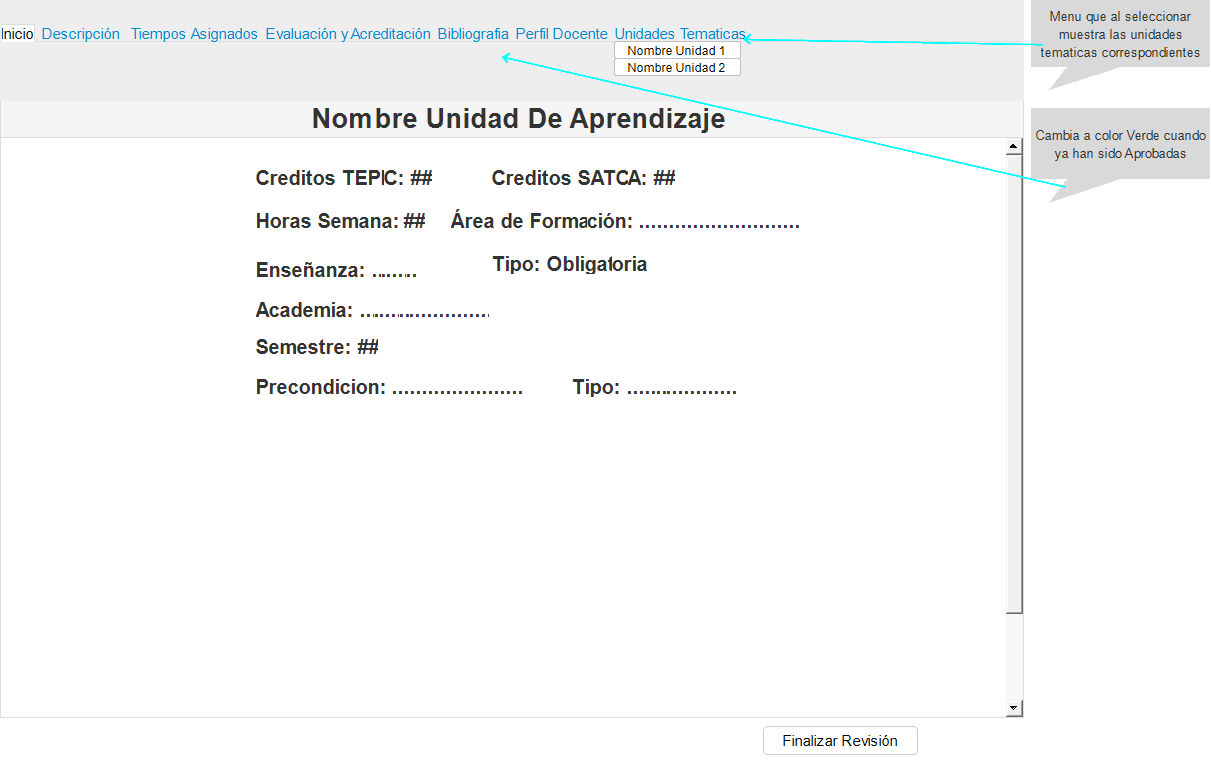
\includegraphics[width=0.7\textwidth]{DCU/SP2/Pantallas/Inicio}
  \caption{SP2-IU-INICIO}
  \label{SP2-IU-INICIO}
\end{figure}

\begin{figure}
  \centering
    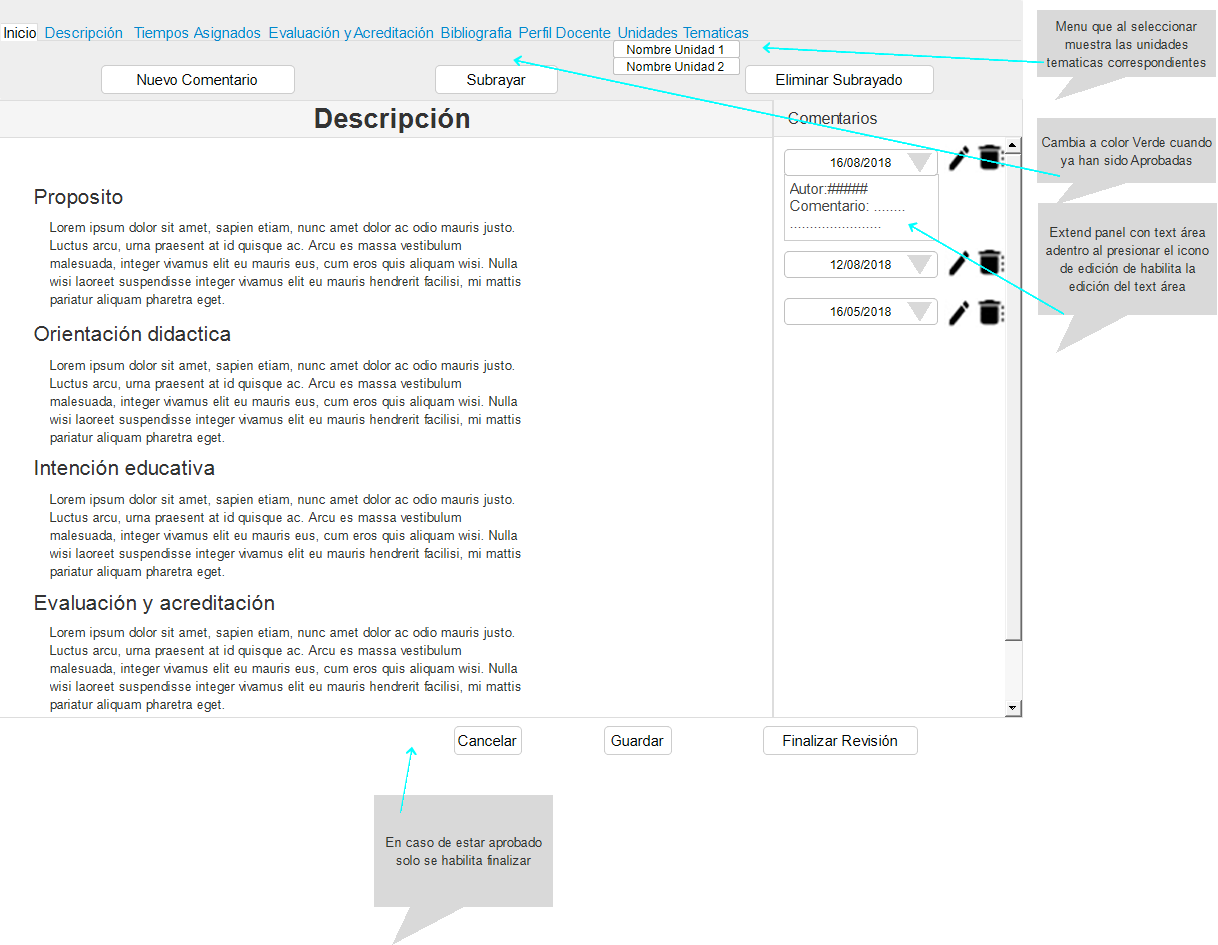
\includegraphics[width=0.7\textwidth]{DCU/SP2/Pantallas/Descripcion}
  \caption{SP2-IU-DESCRIPCION}
  \label{SP2-IU-DESCRIPCION}
\end{figure}

